%%%%%%%%%%%%%%%%%%%%%%%%%%%%%%%%%%%%%%%%%
% University/School Laboratory Report
% LaTeX Template
% Version 3.1 (25/3/14)
%
% This template has been downloaded from:
% http://www.LaTeXTemplates.com
%
% Original author:
% Linux and Unix Users Group at Virginia Tech Wiki 
% (https://vtluug.org/wiki/Example_LaTeX_chem_lab_report)
%
% License:
% CC BY-NC-SA 3.0 (http://creativecommons.org/licenses/by-nc-sa/3.0/)
%
%%%%%%%%%%%%%%%%%%%%%%%%%%%%%%%%%%%%%%%%%

%----------------------------------------------------------------------------------------
%	PACKAGES AND DOCUMENT CONFIGURATIONS
%----------------------------------------------------------------------------------------

\documentclass[11pt,a4paper]{article}

\usepackage[version=3]{mhchem} % Package for chemical equation typesetting
\usepackage{siunitx} % Provides the \SI{}{} and \si{} command for typesetting SI units
\usepackage{graphicx} % Required for the inclusion of images
\usepackage{natbib} % Required to change bibliography style to APA
\usepackage{amsmath} % Required for some math elements 

% Fall mal eigene margins definiert werden müssen
%\usepackage{geometry}
% \geometry{
% a4paper,
% total={170mm,257mm},
% left=20mm,
% top=20mm,
% }
% 
\setlength\parindent{0pt} % Removes all indentation from paragraphs

\renewcommand{\labelenumi}{\alph{enumi}.} % Make numbering in the enumerate environment by letter rather than number (e.g. section 6)

%\usepackage{times} % Uncomment to use the Times New Roman font

%----------------------------------------------------------------------------------------
%	DOCUMENT INFORMATION
%----------------------------------------------------------------------------------------

\title{CPA Lab-Report \\ Lab 2 Prime Numbers} % Title

\author{Simon \textsc{Birrer}, Dominic \textsc{Sch\"urmann}} % Author name

\date{\today} % Date for the report

\begin{document}

\maketitle % Insert the title, author and date

\begin{center}
\begin{tabular}{l r}
Date Performed: & October 27, 2015 \\ % Date the experiment was performed
Partners: & Simon Birrer \\ % Partner names
& Dominic Sch\"umann \\
Instructor: & Professor Smith % Instructor/supervisor
\end{tabular}
\end{center}

\bigskip

\tableofcontents

\pagebreak

\section{Biggest prime storable in 8 bytes}

The Source for the solution is in the file \textit{primo\textunderscore  grande.c} 

\subsection{Compiling without OpenMP}

To use the program in both ways, either with or without OpenMP , we used the preproccessor directives. Now the compiler decides upon the arguments if the code will use OpenMP or not.\\

ToDo insert code sample


\subsection{Time measurement of parallelized version}

\begin{figure}[ht]
\centering
  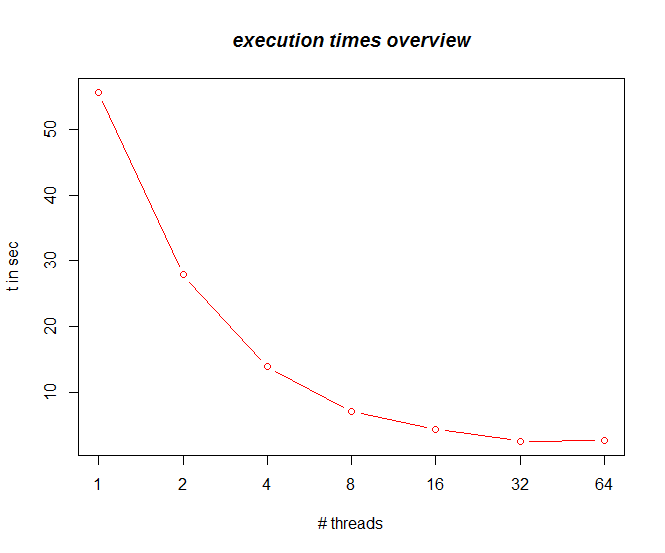
\includegraphics[scale=0.35]{statistics/Ex12ResultGraph.png}
	\caption{execution times for exercise 1.2}
	\label{ex12execution}
\end{figure}



In figure \ref{ex12execution} are the measured times of executing the program with different numbers of threads using kahan.\\

Since a node of kahan has 32 cores, the execution with 32 threads was the fastest. In addition the performance decreases if the number of threads will be increased. This is shown in figure \ref{ex12execution} and the overhead is even more visible in figure \ref{ex12speedUp} .

\begin{figure}[ht]
\centering
  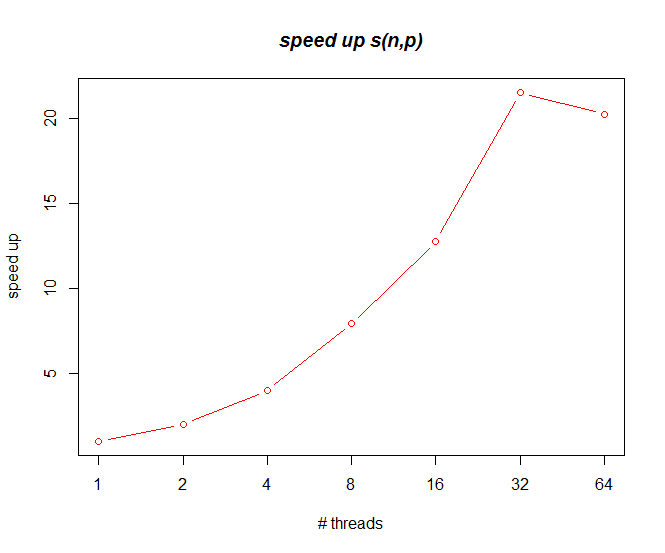
\includegraphics[scale=0.35]{statistics/Ex12SpeedUpGraph.png}
	\caption{speed up for exercise 1.2}
	\label{ex12speedUp}
\end{figure}



\pagebreak

\section{Count primes in a range}

The Source for the solution of exercise \ref{ex21} is in the file
 \textit{primo\textunderscore numeros\textunderscore 1.c} and
 for exercise \ref{ex22} in file \textit{primo\textunderscore numeros\textunderscore 2.c}

\subsection{Exercise 1 with reduction clause}
\label{ex21}
\subsubsection{scheduling distribution}


\begin{itemize}
\item static 0, without chunk
\item static 1, with chunk
\item dynamic
\end{itemize}

\subsection{Exercise 2 printing workload}
\label{ex22}

%----------------------------------------------------------------------------------------
%	BIBLIOGRAPHY
%----------------------------------------------------------------------------------------

\bibliographystyle{apalike}

\bibliography{sample}

%----------------------------------------------------------------------------------------


\end{document}